\begin{frame}
  \frametitle{A Web Application}
  % facilitate the usage for non-developer end-users
  % what it does, see readme
  % it is intuitive
  % As a backend, it uses a minimalistic and efficient python web framework: flask
  % it's in active development
\end{frame}

\begin{frame}
  \frametitle{About Flask}
  % search the internet and explain the concept here
  % put a simple example of code (the one they provide in the quickstart of the
  % doc)

  \begin{itemize}
    \item micro web framework for Python;
    \item handy to launch small applications or web page
  \end{itemize}

The following code aims at displaying "Hello World!" on a web page: 

  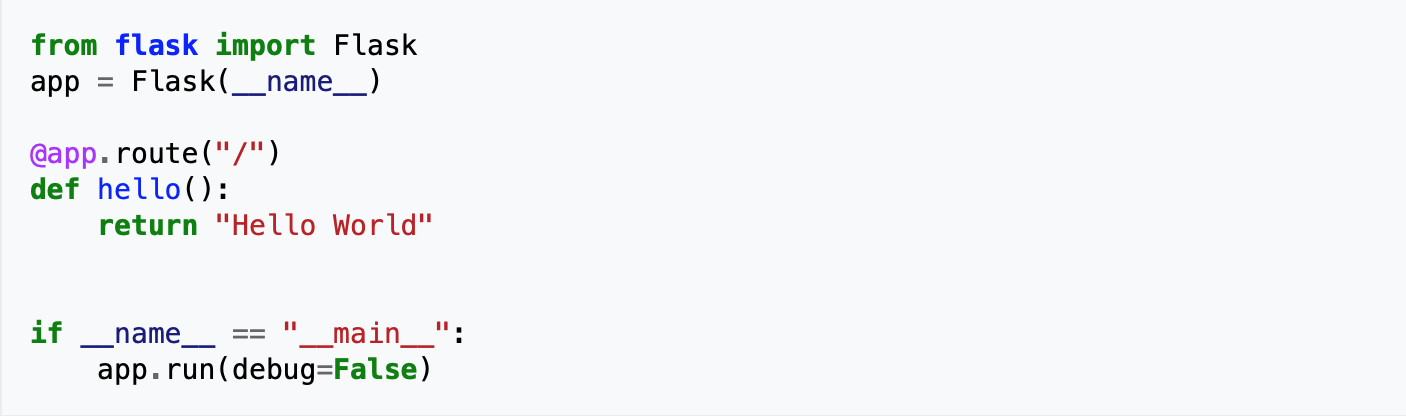
\includegraphics[scale=0.4]{../inc/graphics/flask.png}

\end{frame}
